\documentclass[runningheads]{llncs}
\usepackage[T1]{fontenc}
\usepackage{graphicx}
\usepackage{booktabs}
\usepackage{amsmath,amssymb}
\usepackage{url}

\title{Auto-Decte: Trust-Constrained Human-in-the-Loop Document Intelligence via Candidate-Fact Separation}
\titlerunning{Trust-Constrained Document Intelligence}

\author{Anonymous Authors}
\institute{Anonymous Institution}

\begin{document}
\maketitle

\begin{abstract}
High-stakes document extraction requires control over how machine outputs become authoritative records, not only high recognition accuracy. A single transcription error in a payroll-adjacent form can affect a worker's wage, while a conventional automated pipeline may propagate that error without an explicit decision. We present a trust-constrained human-in-the-loop framework based on \emph{candidate-fact separation}, instantiated in Auto-Decte for structured industrial paper forms. Every output from perception, a large language model (LLM), or retrieval is stored as an append-only candidate or a read-only reference; only an explicit human decision creates or updates a versioned fact. Recognition also abstains on uncertain cells and routes them to review. Auto-Decte combines QR-based template identification, ArUco-based perspective correction, selective digit and OMR recognition, an optional DeepSeek adapter, local retrieval, and an offline-capable progressive web application. On controlled synthetic benchmarks, the conservative recognition threshold yields 100\% accuracy among accepted predictions at 61.4\% coverage, while clean whole-form cell accuracy is 97.5\%. A suite of 478 automated tests exercises evidence integrity, candidate isolation, human-only fact transitions, traceability, and operation with the LLM disabled. These results characterize the accuracy--coverage trade-off while the architecture establishes a narrower guarantee: machine modules have no direct write path to the fact plane.
\end{abstract}

\keywords{trustworthy document intelligence \and candidate-fact separation \and selective prediction \and human-in-the-loop \and knowledge extraction \and trustworthy data mining}

\section{Introduction}
Foundation-model-assisted document processing is attractive for the long tail of paper-based workflows in small and medium-sized plants, but payroll-adjacent settings require more than high average accuracy. An incorrectly transcribed digit can affect a worker's wage, and a retrieved historical record can be mistaken for current evidence. Fully automated pipelines can therefore propagate consequential errors, whereas purely manual digitization is difficult to scale. This motivates our central research question: \emph{how can machine perception and generative assistance support high-risk document extraction without giving machine-generated content a direct path into the authoritative data layer?}

We address this with a trust-constrained framework whose two principles are (i) \emph{candidates, never facts}, and (ii) \emph{abstention over guessing}. We study three sub-problems: (RQ1) reducing perception uncertainty on structured paper forms (template-guided perception with an explicit ambiguity band); (RQ2) letting LLM/RAG provide assistance without contaminating facts (candidate/reference isolation); (RQ3) making human confirmation the sole path that writes facts while preserving traceability (append-only candidates, versioned decisions, evidence lineage).

\textbf{Positioning.} Existing approaches address complementary parts of this problem: OCR and document understanding optimize extraction quality; human-in-the-loop systems add review to machine prediction; and LLM/RAG systems provide semantic suggestions or retrieve supporting material. These capabilities do not by themselves impose a data-model constraint on how machine output reaches an authoritative record. Auto-Decte treats every machine output as a candidate or reference, abstains on uncertain predictions, and reserves fact creation and revision for explicit human actions. The contribution is therefore an enforced architectural invariant that combines selective abstention with machine-to-fact isolation, rather than a new OCR, fiducial, LLM, or retrieval algorithm.

Our contributions are:
\begin{enumerate}
\item A \emph{trust-constrained framework} with separate evidence, candidate, human-decision, and fact planes. This design removes direct machine-to-fact write paths.
\item \emph{Selective recognition via abstention}, using a template-matching margin for digits and a fill-ratio rejection band for OMR, together with an evaluation of the coverage--selective-risk trade-off.
\item \emph{Trust-bounded LLM and retrieval assistance}: suggestions remain isolated from confirmed values, retrieval is read-only, and the core workflow remains operational when the LLM is disabled.
\item An offline-capable implementation evaluated for recognition, perturbation robustness, retrieval relevance, end-to-end processing, and architectural invariants.
\end{enumerate}

\section{Related Work}
\textbf{Document understanding.} General document AI systems emphasize extraction quality across diverse layouts. PP-OCRv3 improves an OCR pipeline~\cite{ppocrv3}; LayoutLMv3 learns multimodal document representations~\cite{layoutlmv3}; and Donut performs OCR-free document understanding~\cite{donut}. SurveyNet~\cite{surveynet} combines OCR and OMR for survey digitization. Auto-Decte instead targets fixed, structured forms and governs the transition from extracted values to authoritative records.

\textbf{Fiducial localization and human review.} ArUco detection~\cite{aruco} and marker dictionaries constructed by mixed-integer linear programming~\cite{milp} provide the geometric anchors used for deterministic template recovery. Active-learning and human-in-the-loop research~\cite{budd} motivates targeted review, often as a means of improving a model or correcting its predictions. Our design assigns review a different architectural role: an explicit human action is required for every fact transition.

\textbf{LLM/RAG assistance and selective prediction.} Work on generative information extraction~\cite{llmgie}, retrieval-augmented generation~\cite{rag}, and local-first software~\cite{localfirst} informs the optional assistant, reference retrieval, and offline submission path. Abstention originates in Chow's reject option~\cite{chow}, has been studied for deep selective classification~\cite{geifman}, and is related to distribution-free uncertainty quantification~\cite{angelopoulos}. We apply abstention to per-cell structured-form extraction and combine it with a machine-to-fact isolation boundary. The individual components are established; the contribution lies in their integration as an enforced trust architecture.

\section{Problem Formulation and Design Principles}
\textbf{High-risk document extraction.} A paper form is photographed and mapped to structured field values $y=\{y_j\}$. In addition to accurate predictions $\hat y_j$, the system must ensure that no machine-generated value can modify the authoritative record without an explicit and attributable human action.

\textbf{Candidate versus fact.} The design uses evidence, candidate, and fact planes separated by a human trust boundary. The \emph{evidence plane} holds immutable, content-addressed inputs, including SHA-256-addressed images. The \emph{candidate plane} holds recognition hypotheses, LLM suggestions, and retrieval references. Candidates are append-only and cannot overwrite facts. The \emph{fact plane} contains versioned values created or revised only when a human confirms or corrects a candidate. This separation is enforced by the data model.

\textbf{Abstention over guessing.} The recognizer returns a value only when its confidence satisfies the acceptance rule; otherwise, it returns an explicit abstention and routes the cell to review. Abstention is therefore a first-class output rather than an exception handled after prediction.

\textbf{Trust model.} Let $E$, $C$, $H$, and $F$ denote the evidence, candidate, human-decision, and fact planes. Every machine module $m\in M$ (perception, LLM, or retrieval) may write only to $C$; the fact plane evolves solely through human decisions, $F_{t+1}=g(F_t,H_t)$. The invariant $\forall m\in M: m\not\rightarrow F$ states that no machine module has a direct write path to the fact plane. This architectural property is distinct from empirical recognition accuracy. It does not guarantee that a reviewer will identify every incorrect candidate; it guarantees that every fact transition is explicit, attributable to a human decision, and traceable to its evidence and candidates.

Figure~\ref{fig:isolation} makes this separation explicit: machine components terminate at the candidate plane, whereas the only transition into the fact plane crosses the human trust boundary.

\begin{figure}[t]
\centering
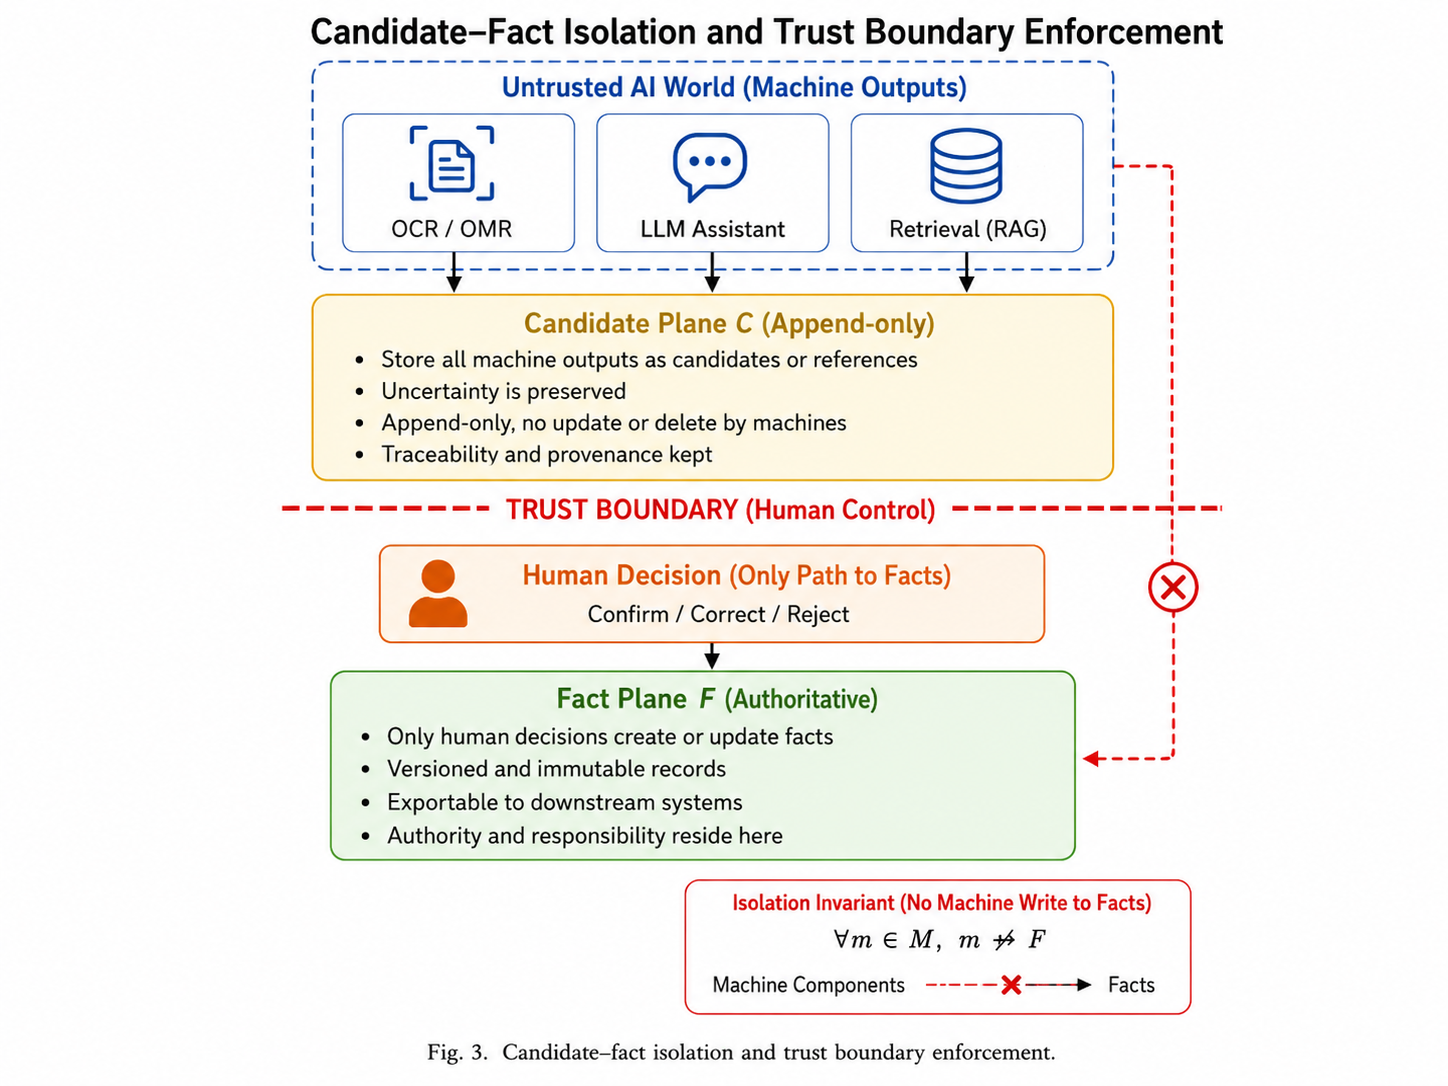
\includegraphics[width=0.94\textwidth,trim=0 55 0 0,clip]{../figures/candidate_fact_isolation.png}
\caption{Candidate--fact isolation and trust-boundary enforcement. Machine modules may append candidates or supply read-only references, but they cannot directly create or update authoritative facts.}
\label{fig:isolation}%
\end{figure}

\section{Trust-Constrained Document Intelligence}
\textbf{Template-guided perception.} Templates contain a QR code encoding identity and version and ArUco corner markers with IDs 10--13. A multi-region QR search identifies the form, four ArUco markers map the image to a canonical canvas by perspective correction, and the system crops fields according to the corresponding template definition. This deterministic and auditable geometry reduces recognition to per-cell decisions.

\textbf{Selective recognition with a rejection region.} Digit cells are normalized to $48{\times}64$, binarized with Otsu's method, and compared with ten rendered synthetic-font templates using normalized mean absolute difference. Let $d_1(x)$ and $d_2(x)$ denote the smallest and second-smallest template distances. The margin $s(x)=d_2(x)-d_1(x)$ defines the decision rule
\begin{equation}
D(x)=
\begin{cases}
\hat y, & s(x)\geq\tau,\\
\textsc{Abstain}, & s(x)<\tau.
\end{cases}
\end{equation}
Cells with an ink ratio below 1\% are reported as blank. Checkbox (OMR) cells use an interior fill ratio: values at or below 0.15 are unchecked, values at or above 0.35 are checked, and values in $(0.15,0.35)$ trigger abstention.

\textbf{Candidate isolation.} Recognition attempts and LLM suggestions are stored as append-only candidates linked to their evidence; retrieval results are stored as read-only references. Neither can overwrite a confirmed value. The DeepSeek adapter uses structured output and is disabled by default, while the core pipeline runs end-to-end without the model.

\textbf{Read-only retrieval.} A local, dependency-free similarity index based on character bigrams and word-level cosine similarity surfaces related historical forms. Retrieved items are references only and cannot participate in a fact update.

\textbf{Human decision layer.} A React review workbench is the sole interface for moving from candidates to facts. Operators confirm or correct values under rule validation. Each action appends a versioned record and a before--after audit pair, allowing an exported value to be traced to its form, version, evidence, and event log.

Figure~\ref{fig:pipeline} summarizes the operational path from evidence acquisition and template-guided recognition to selective routing, human review, and export.

\begin{figure}[t]
\centering
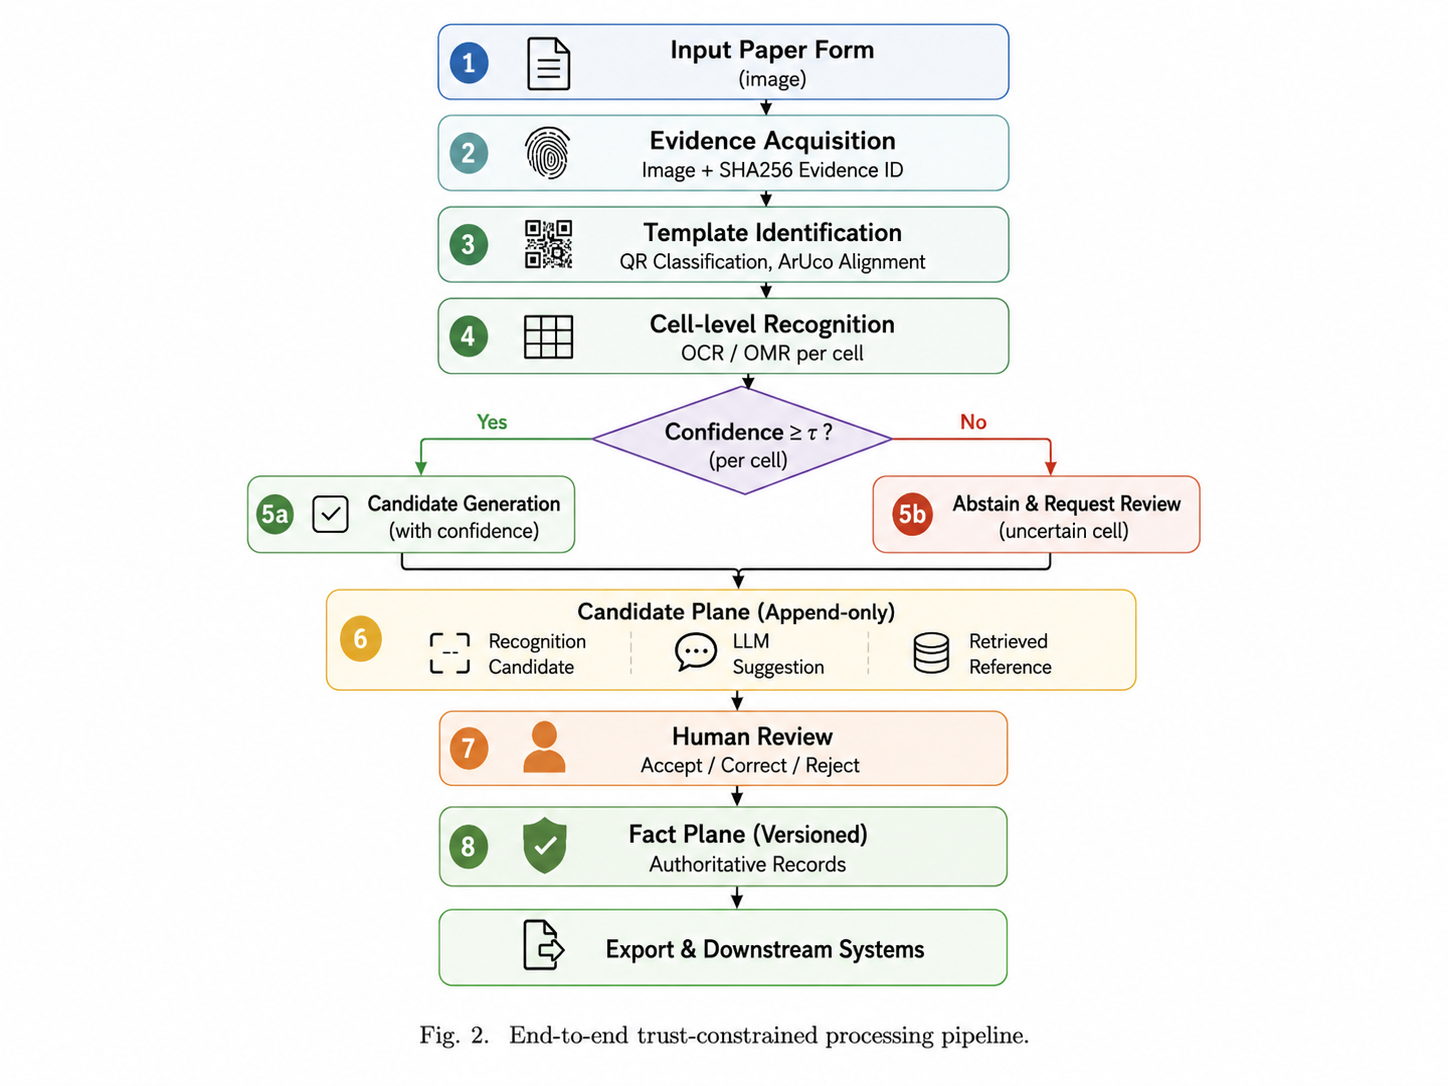
\includegraphics[width=0.94\textwidth,trim=0 90 0 0,clip]{../figures/processing_pipeline.png}
\caption{End-to-end trust-constrained processing pipeline. Low-confidence cells trigger abstention and review; accepted predictions remain candidates until a human decision creates a versioned fact.}
\label{fig:pipeline}%
\end{figure}

\section{System Architecture}
Auto-Decte instantiates the design as four logically separated planes: evidence, candidates, human decisions, and facts. Figure~\ref{fig:arch} shows how the untrusted machine components connect to these planes. The evidence plane stores SHA-256-addressed images. The candidate plane contains append-only recognition attempts and LLM suggestions, alongside read-only retrieval references. The review workbench implements the human trust boundary. The fact plane stores versioned records, audit events, and export batches under role-based access for operators, reviewers, finance staff, administrators, and auditors. A progressive web application (PWA) uses an IndexedDB outbox to route offline plant-floor submissions into the same review queue. Authentication and request integrity rely on scrypt-derived credentials, HttpOnly cookies, double-submit CSRF protection, and idempotency keys.

\begin{figure}[t]
\centering
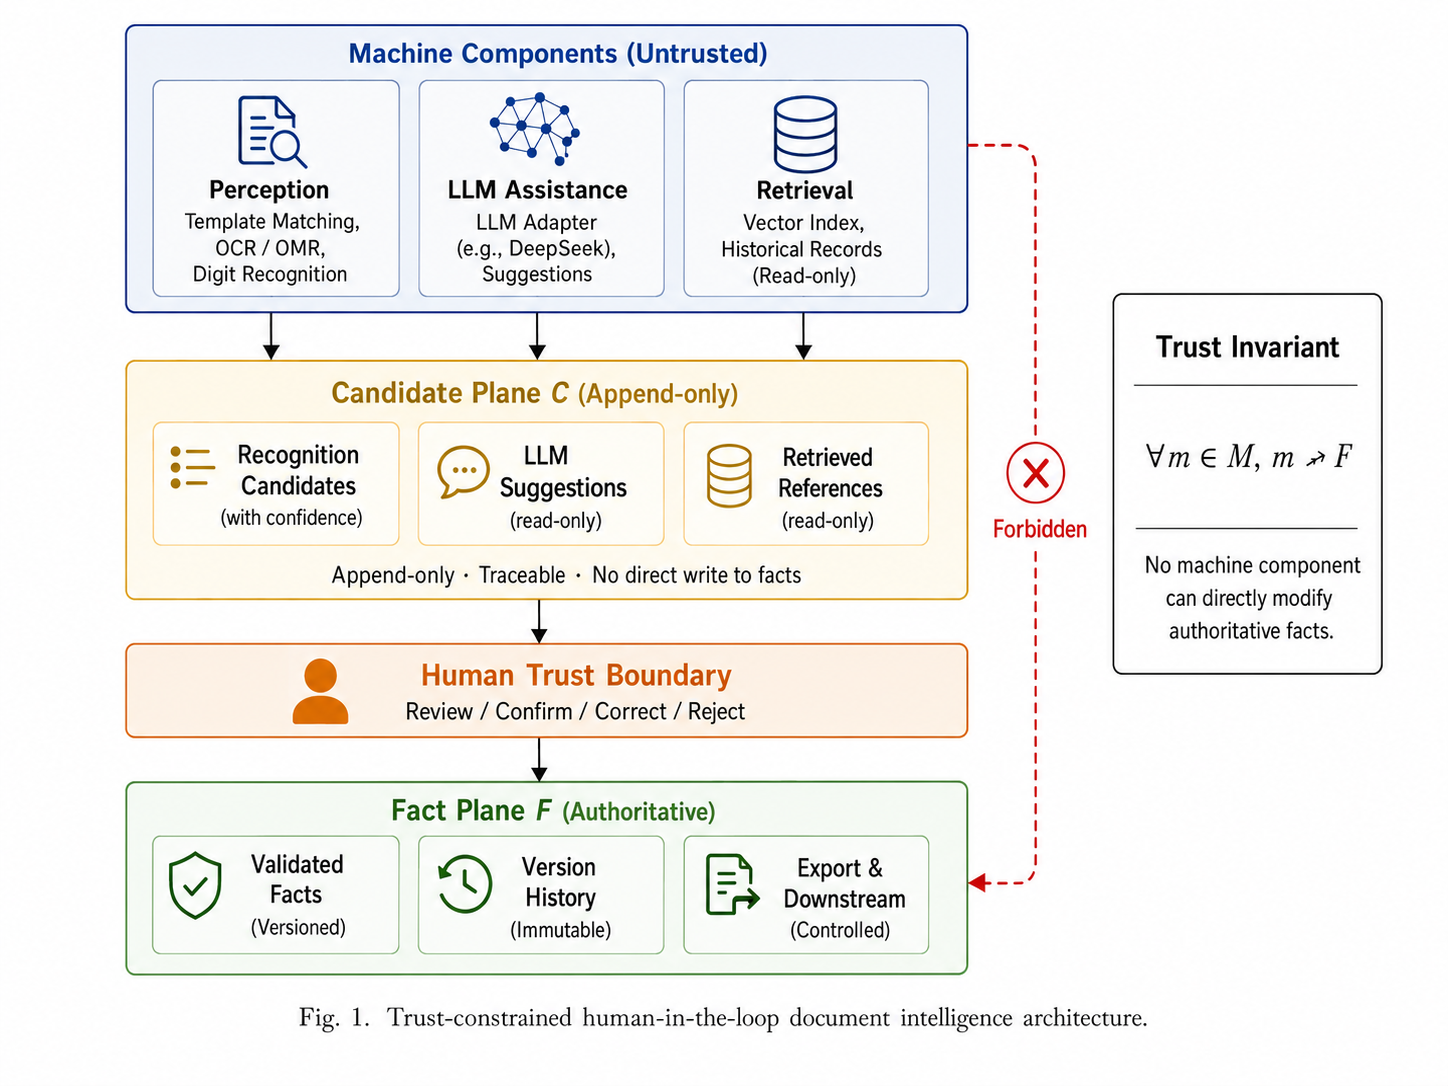
\includegraphics[width=0.94\textwidth,trim=0 90 0 0,clip]{../figures/trust_architecture.png}
\caption{Trust-constrained architecture of Auto-Decte. Perception, LLM assistance, and retrieval terminate at append-only candidates or read-only references. The human trust boundary is the only path to versioned facts.}
\label{fig:arch}%
\end{figure}

\section{Implementation}
The FastAPI backend runs on Python 3.11. The persistence layer uses SQLite, SQLAlchemy 2.0, and Alembic migrations. The front end uses React~18 and Vite, image operations use OpenCV, the optional suggestion service uses a DeepSeek client, and retrieval uses a local similarity index. The evaluated V1 implementation passes 478 automated tests, including acceptance tests for evidence integrity, trust-boundary enforcement, review workflows, and audit traceability.

\section{Experimental Evaluation}

\subsection{Methodology and Research-Question Mapping}
The evaluation comprises five components: functional acceptance tests; controlled recognition benchmarks on synthetic filled forms under blur, rotation, brightness variation, Gaussian noise, and perspective tilt; comparisons with a learned recognizer and a general OCR baseline; retrieval precision on a synthetic corpus; and a sweep of the selective-prediction threshold. We organize these components around the three research questions in Section~1.

\subsection{RQ1: Can Selective Recognition Reduce Unreviewed Errors?}
Sweeping the margin threshold $\tau$ yields the coverage--risk curve in Fig.~\ref{fig:coverage} and Table~\ref{tab:selective}. At the operating point $\tau=0.02$, the system covers 93.7\% of cells with 94.7\% accuracy among accepted predictions, corresponding to 5.3\% selective risk. At $\tau=0.05$, accepted-prediction accuracy reaches 100\% on this benchmark, with 61.4\% coverage; the remaining 38.6\% of cells are routed to review. Thus, no error is observed among predictions accepted at the conservative threshold, although this result does not establish zero risk beyond the benchmark distribution.

The baselines clarify the scope of this trade-off. A HOG + linear-SVM recognizer attains 100\% accuracy on the printed font and 79.7--80.3\% on unseen fonts, but it has no abstention output. In single-character mode, Tesseract attains 84--87\% on the deployment-relevant printed-template regime, compared with 100\% for the template matcher. Tesseract performs better on unseen fonts (94--95\% versus 86--90\%), which lie outside the intended printed-form scope. Among the evaluated recognizers, only the template matcher exposes an explicit ambiguity channel.

\begin{figure}[t]
\centering
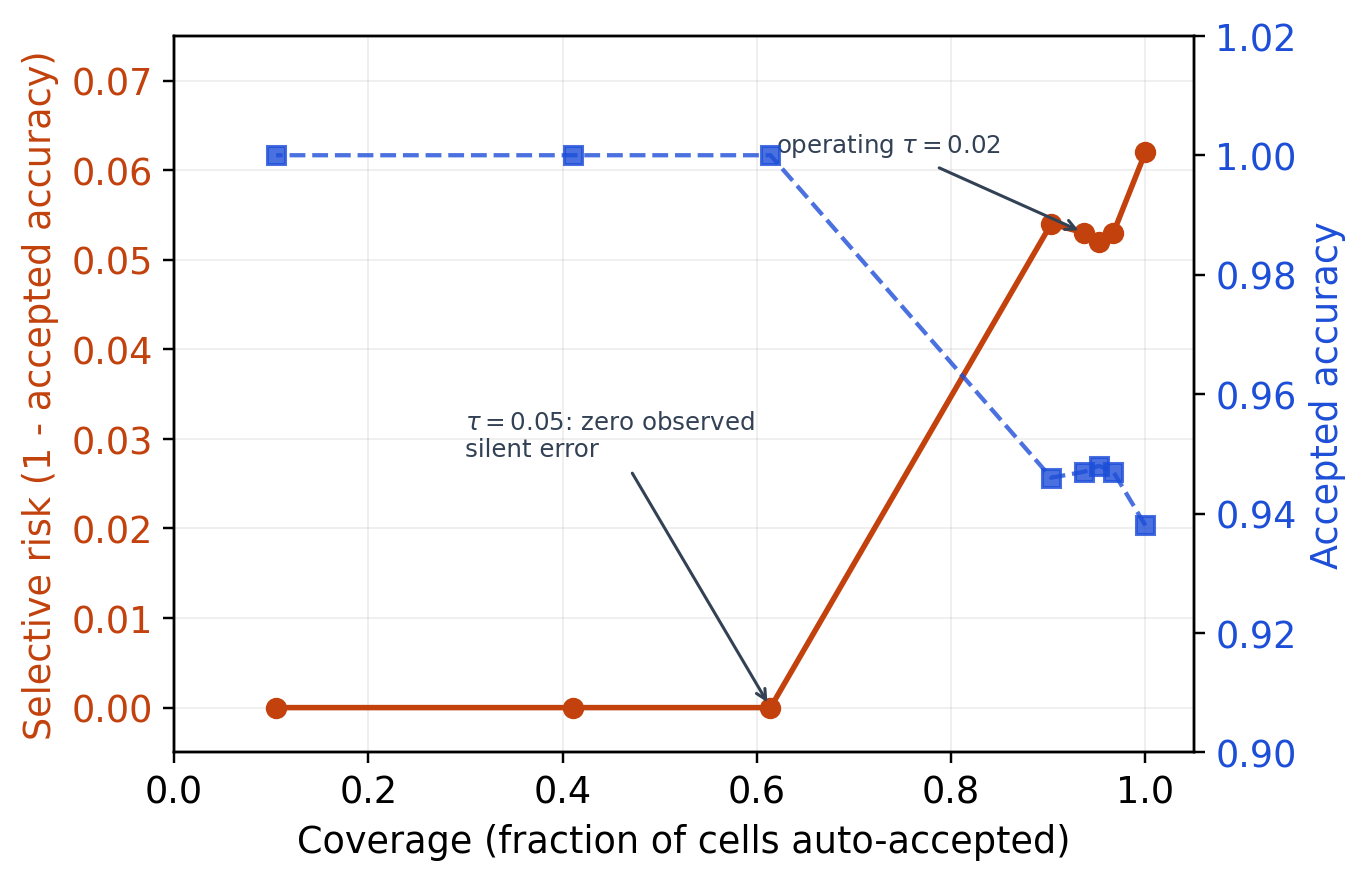
\includegraphics[width=0.85\textwidth]{../figures/coverage_risk.png}
\caption{Coverage versus selective risk over the abstention threshold. Increasing $\tau$ lowers coverage; the observed selective risk reaches zero at the conservative thresholds on this controlled benchmark. The operating point $\tau=0.02$ is marked.}
\label{fig:coverage}%
\end{figure}

\begin{table}[b]
\centering
\caption{Selective recognition: full sweep of coverage vs selective risk over the abstention threshold $\tau$.}
\label{tab:selective}%
\begin{tabular}{lcccc}
\toprule
$\tau$ & Coverage & Accepted acc. & Selective risk & Routing rate \\
\midrule
0.000 (always guess) & 1.000 & 0.938 & 0.062 & 0.000 \\
0.005 & 0.967 & 0.947 & 0.053 & 0.033 \\
0.010 & 0.952 & 0.948 & 0.052 & 0.048 \\
0.020 (operating) & 0.937 & 0.947 & 0.053 & 0.063 \\
0.030 & 0.903 & 0.946 & 0.054 & 0.097 \\
0.050 (conservative) & 0.614 & 1.000 & 0.000 & 0.386 \\
0.080 (conservative) & 0.411 & 1.000 & 0.000 & 0.589 \\
0.120 & 0.105 & 1.000 & 0.000 & 0.896 \\
\bottomrule
\end{tabular}
\end{table}

\subsection{RQ2: Does the Trust Boundary Block Direct Machine-to-Fact Writes?}
We inject an incorrect LLM suggestion into a form that already has a confirmed record. The confirmed fact remains unchanged, the suggestion is stored separately as a candidate, and no record version contains the injected value. A later human correction becomes the next authoritative version. This experiment directly exercises the LLM-suggestion path. The data model applies the same candidate-plane write restriction to recognition output, while retrieval output remains read-only. The acceptance suite also verifies that the workflow completes with the LLM disabled and that exports can be traced to their supporting records and evidence.

We evaluate retrieval on a synthetic corpus of 200 records from five templates, defining relevance as a shared template key. Mean precision is 1.00 at rank 1, 0.99 at rank 3, 0.975 at rank 5, and 0.95 at rank 10. These values are expected to be high because the template key is a distinctive lexical token. The experiment therefore checks that useful references are surfaced; candidate-fact isolation, rather than retrieval precision, provides the trust property.

\subsection{RQ3: How Robust Is Perception under Controlled Perturbations?}
Digit recognition achieves 93.9\% aggregate accuracy across 28 font--perturbation conditions. Accuracy is 100\% for the printed template font under blur, rotation, noise, and brightness variation, and 80--90\% for unseen fonts, for which 10--20\% of cells are rejected. OMR decisions are 100\% correct outside the rejection band, while all samples inside the band trigger abstention. The 93.9\% aggregate pertains to single-digit-cell conditions and is distinct from the whole-form metric reported below.

QR recovery succeeds for all 90 perturbed renders. ArUco correction succeeds for all clean, blurred, noisy, brightness-adjusted, and perspective-tilted images, with at most 0.34\,px alignment error. Success falls to 50\% at $3^\circ$ rotation and 20\% at $5^\circ$. For end-to-end synthetic forms containing 10 digit cells and 10 OMR boxes, cell-level accuracy is 97.5\% on clean images and 96.5--98.0\% under blur, noise, brightness variation, and perspective tilt; 4.5--8.5\% of digit cells are rejected. At $3^\circ$ rotation, correction success falls to 60\%. Per-image stage latency is 2{,}180\,ms for QR search, 20\,ms for quality assessment, and 35\,ms for geometric correction.

\textbf{LLM/RAG assistance.} The present evaluation tests isolation and functional correctness rather than reviewer efficiency. Reviewer time, error-detection rate, and suggestion-acceptance rate remain to be measured in the planned field pilot described in Section~8.

\section{Industrial Case Study}
Auto-Decte operates as a working baseline at a bamboo-processing plant, where it supports the transition from handwritten payroll and production records to a reviewable digital workflow. This deployment demonstrates operational feasibility in the target setting. The quantitative results in Section~6, however, come from controlled and reproducible benchmarks because production records are excluded from the public repository. We therefore make no claim about the deployment's effect on processing time, cost, or error rates; the deployment motivates the design and provides the setting for a future field pilot.

\section{Scope and Limitations}
This paper addresses \emph{structured printed industrial forms}, the regime for which template-guided perception was designed, rather than general-purpose document understanding. Several limitations remain. First, the system does not recognize general handwriting, Chinese text, or signatures; perception is limited to single-cell printed digits and OMR\@. Second, the current deployment is single-machine and has not undergone a multi-user capacity test. Third, the evaluation uses controlled synthetic benchmarks rather than a double-entered reference set of real plant images, so the accuracy results should not be extrapolated beyond the tested conditions. Fourth, the study does not measure whether LLM or retrieval assistance improves review efficiency. Future work will integrate broader OCR, add independent task workers, compare recognition-only, retrieval-assisted, and LLM-assisted review, and conduct a field pilot measuring processing time and error outcomes.

\section{Conclusion}
The Auto-Decte framework assigns perception and LLM output to candidates, keeps retrieval references read-only, and requires an explicit human action to create or revise a fact. The controlled evaluation quantifies the trade-off between coverage and selective risk: a conservative threshold produces no observed error among accepted predictions on the benchmark, but routes 38.6\% of cells to review. The system also preserves traceability and remains operational with the LLM disabled. Auto-Decte therefore does not assume that every machine prediction is correct. Instead, it restricts when predictions are accepted and prevents machine modules from writing directly to authoritative records. Evaluation on real production forms and measurement of reviewer efficiency remain necessary before claims about field effectiveness can be made.

\bibliographystyle{splncs04}
\begin{thebibliography}{99}
\bibitem{ppocrv3} C.~Li et al.: PP-OCRv3: More attempts for the improvement of ultra lightweight OCR system. arXiv:2206.03001 (2022)
\bibitem{layoutlmv3} Y.~Huang, T.~Lv, L.~Cui, Y.~Lu, F.~Wei: LayoutLMv3: Pre-training for document AI with unified text and image masking. In: ACM MM, 4083--4091 (2022). doi:10.1145/3503161.3548112
\bibitem{donut} G.~Kim et al.: OCR-free document understanding transformer. In: ECCV, LNCS 13688, 498--517 (2022). doi:10.1007/978-3-031-19815-1\_29
\bibitem{surveynet} R.~Qui{\~n}ones, S.~Cheekireddy, E.~Gultepe: SurveyNet: A unified deep learning framework for OCR and OMR-based survey digitization. J. Imaging 12(4), 175 (2026). doi:10.3390/jimaging12040175
\bibitem{aruco} F.J.~Romero-Ramirez, R.~Mu{\~n}oz-Salinas, R.~Medina-Carnicer: Speeded up detection of squared fiducial markers. Image Vis. Comput. 76, 38--47 (2018). doi:10.1016/j.imavis.2018.05.004
\bibitem{milp} S.~Garrido-Jurado, R.~Mu{\~n}oz-Salinas, F.J.~Madrid-Cuevas, R.~Medina-Carnicer: Generation of fiducial marker dictionaries using mixed integer linear programming. Pattern Recognit. 51, 481--491 (2016). doi:10.1016/j.patcog.2015.09.023
\bibitem{budd} S.~Budd, E.C.~Robinson, B.~Kainz: A survey on active learning and human-in-the-loop deep learning for medical image analysis. Medical Image Analysis 71, 102062 (2021)
\bibitem{chow} C.K.~Chow: On optimum recognition error and reject tradeoff. IEEE Transactions on Information Theory 16(1), 41--46 (1970)
\bibitem{geifman} Y.~Geifman, R.~El-Yaniv: Selective classification for deep neural networks. In: NeurIPS (2017)
\bibitem{angelopoulos} A.N.~Angelopoulos, S.~Bates: Conformal prediction: A gentle introduction. Found. Trends Mach. Learn. 16(4), 494--591 (2023). doi:10.1561/2200000101
\bibitem{llmgie} D.~Xu et al.: Large language models for generative information extraction: A survey. Front. Comput. Sci. 18(6), 186357 (2024). doi:10.1007/s11704-024-40555-y
\bibitem{rag} Y.~Gao et al.: Retrieval-augmented generation for large language models: A survey. arXiv:2312.10997 (2023)
\bibitem{localfirst} M.~Kleppmann, A.~Wiggins, P.~van Hardenberg, M.~McGranaghan: Local-first software: You own your data, in spite of the cloud. In: Onward! (2019). doi:10.1145/3359591.3359737
\end{thebibliography}

\end{document}
